\hypertarget{ux5b9eux6218}{%
\subsection{实战}\label{ux5b9eux6218}}

看完了教程,是不是有这么一种感觉:看的时候觉得很简单,照着教程敲代码也没啥大问题。

于是准备开始独立写代码,就发现不知道从哪开始下手了。

这种情况是完全正常的。好比学写作文,学的时候觉得简单,写的时候就无从下笔了。

虽然这个教程是面向小白的零基础 Python 教程,但是我们的目标不是学到 60
分,而是学到 90 分。

所以,用 Python 写一个真正的 Web App 吧!

\hypertarget{ux76eeux6807}{%
\subsubsection{目标}\label{ux76eeux6807}}

我们设定的实战目标是一个 Blog 网站,包含日志、用户和评论 3 大部分。

很多童鞋会想,这是不是太简单了?

比如 \href{http://webpy.org/src/blog/0.3}{webpy.org} 上就提供了一个 Blog
的例子,目测也就 100 行代码。

但是,这样的页面:

 
 \begin{figure}[htp]
	\centering
	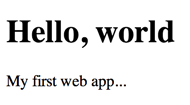
\includegraphics[width=0.6\linewidth]{fig/954926361167104.png}
\end{figure}


你拿得出手么?

我们要写出用户真正看得上眼的页面,首页长得像这样:

 
 \begin{figure}[htp]
	\centering
	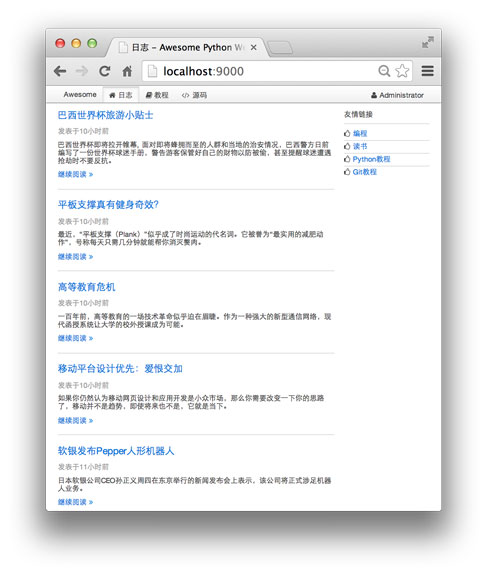
\includegraphics[width=0.6\linewidth]{fig/954926929668576.png}
\end{figure}


评论区:

 
 \begin{figure}[htp]
	\centering
	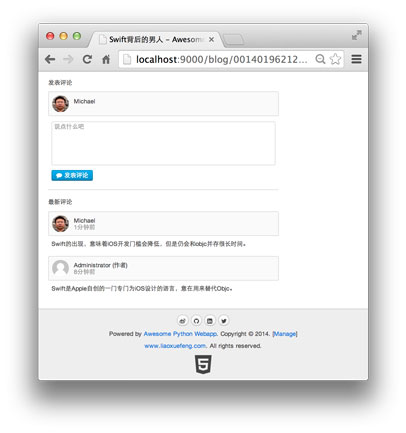
\includegraphics[width=0.6\linewidth]{fig/954926987474240.png}
\end{figure}


还有极其强大的后台管理页面:

 
 \begin{figure}[htp]
	\centering
	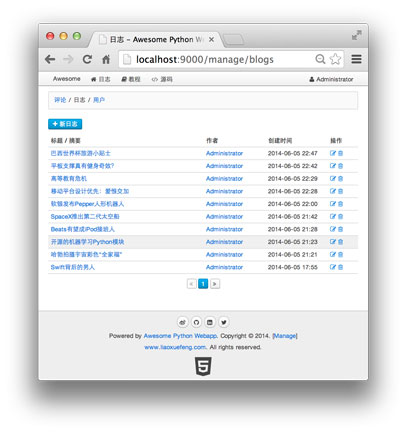
\includegraphics[width=0.6\linewidth]{fig/954927046197152.png}
\end{figure}


是不是一下子变得高端大气上档次了?

\hypertarget{ux9879ux76eeux540dux79f0}{%
\subsubsection{项目名称}\label{ux9879ux76eeux540dux79f0}}

必须是高端大气上档次的名称,命名为\texttt{awesome-python3-webapp}。

\hypertarget{ux9879ux76eeux8ba1ux5212}{%
\subsubsection{项目计划}\label{ux9879ux76eeux8ba1ux5212}}

项目计划开发周期为 16
天。每天,你需要完成教程中的内容。如果你觉得编写代码难度实在太大,可以参考一下当天在
GitHub 上的代码。

第 N
天的代码在\texttt{https://github.com/michaelliao/awesome-python3-webapp/tree/day-N}上。比如第
1 天就是:

\url{https://github.com/michaelliao/awesome-python3-webapp/tree/day-01}

以此类推。

要预览\texttt{awesome-python3-webapp}的最终页面效果,请猛击:

\hypertarget{awesome.liaoxuefeng.com}{%
\subsubsection{\texorpdfstring{\href{http://awesome.liaoxuefeng.com/}{awesome.liaoxuefeng.com}}{awesome.liaoxuefeng.com}}\label{awesome.liaoxuefeng.com}}

